\clearpage
\part{API Documentation}

The intention of the \streams framework is to start from a minimal set
of core concepts and allow for building solutions for more complex
problems on top of that. The main part of this report is a description
of the concepts that mainly focus on establishing a data-flow
definition language.

For running data flow experiments defined with the \streams we provide
an introduction into the \streams {\em runtime} environment in Section
\ref{sec:streamsRuntime}.

\bigskip

The remainder of this document includes a comprehensive documentation
of a set of processors that constitute the \streams API. These
elements provide a toolbox for handling various processing steps and
are described in Section \ref{sec:streamAPI}.

%\bigskip
%Finally this appendix includes the full definitions of the containers
%for some of the use cases, e.g. the FACT telescope data, in Section
%\ref{sec:factAPI}.

\begin{appendix}

%\section{\label{sec:factAPI}Processors for FACT Data}
\section{\label{sec:streamsRuntime}The \streams Runtime}
Along with the \streams API, that is provided for implementing custom
streams or processors, the \streams framework provides a runtime
environment for running stream containers.

\subsection{Running Streams - Quickstart}
Designing a simple stream process does not require more than writing
some XML declaration and executing that XML with the stream-runner as
shown in the following figure:

\begin{figure}[h!]
  \centering
  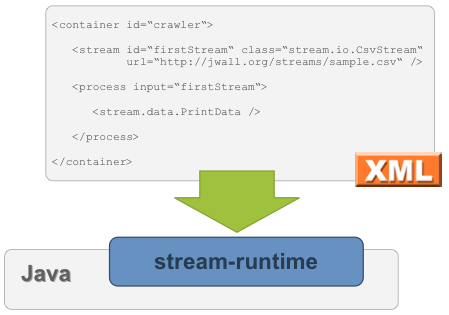
\includegraphics[scale=0.3]{graphics/quickstart-xml}
  \caption{\label{fig:quickstart}Conceptual way of executing a data flow graph that is defined in XML.}
\end{figure}

The simple example presented below, defines a single process that
reads from a CSV stream and prints out the data items to standard
output:

\begin{figure}[h!]
  \centering
  \begin{lstlisting}[language=XML]
    <container>
        <stream id="firstStream" class="stream.io.CsvStream"
                url="http://www.jwall.org/streams/sample-stream.csv" />

        <process input="firstStream">
            <PrintData />
        </process>
     </container>
  \end{lstlisting}
\end{figure}

The {\em stream-runner} required to execute this stream is a simple executable
Java archive available for download:
\begin{displaymath}
  \mbox{\url{http://download.jwall.org/streams/stream-runner.jar}}
\end{displaymath}


\subsubsection{Running a \streams Process}
The simple process defined above can be run by

\hspace{4ex}\sample{\# java -jar stream-runner.jar first-process.xml}

The process will simply read the stream in CSV-format and execute the
processor {\ttfamily PrintData} for each item obtained from the
stream.

\subsubsection{Including additional Libraries}
There exists a set pre-packaged libraries such as {\em streams-analysis}
or {\em streams-video}, which are provided at
\begin{displaymath}
  \mbox{\url{http://download.jwall.org/streams/libs/}}
\end{displaymath}
These add additional processors and stream implementations to the
\streams runtime for different domain specific intentions. To start
the \streams runtime with additional libraries, these need to be
provided on the classpath.

The following example uses the {\ttfamily MJpegImageStream} to process
a stream of video data from some URL. This stream implementation is
provided in the {\em streams-video} package.
\begin{figure}[h!]
  \centering
  \begin{lstlisting}[language=XML]
    <container>
        <stream id="video"
             class="stream.io.MJpegImageStream"
               url="http://download.jwall.org/streams/coffee.mjpeg.gz" />

        <process input="video" >

            <stream.image.DisplayImage key="data" />
            <stream.image.AverageRGB />

            <WithKeys keys="frame:*">
                 <stream.plotter.Plotter
       		         history="1000"
	                keepOpen="true"
	                keys="frame:red:avg,frame:green:avg,frame:blue:avg" />
            </WithKeys>
        </process>
    </container>
  \end{lstlisting}
  \caption{\label{fig:videoExample}Displaying an MJPEG video stream and plotting the average RGB channels.}
\end{figure}

For the libraries to be included in the path, the following command needs
to be issued to start the \streams run-time:

\hspace{4ex}\sample{\# java -cp stream-runner.jar:streams-video-0.0.1.jar $\backslash$
          stream.run video.xml}


\subsection{Installing the \streams Runtime on Debian/RedHat}
For Debian and RPM based systems, there exists a package repository,
that provides Debian and RPM packages that can easily be installed
using the system's package managers. A step-by-step guide for setting
up the package manager on Debian and Ubuntu systems is provided in
Section \ref{sec:installDeb}. Instructions for RedHat based systems
such as RedHat, CentOS or Scientific Linux are provided in
\ref{sec:installRPM}.


\subsubsection{\label{sec:gpgKey}Signatures for Packages}
The repositories and all packages within the repository are
cryptographically signed with a GPG key with ID {\ttfamily 0x13443F4A}
to ensure their consistency. The key is available at

\sample{http://download.jwall.org/software.gpg}

The key is associated with the following information:

\sample{User ID: jwall.org Software Repository <software@jwall.org>\newline
Fingerprint: 175C 915F 51CA 8AA2 387B  E3E8 48E6 B98D 1344 3F4A}

This key needs to be added to the package management key ring of the
system (e.g. {\em apt} on Debian or {\em yum} on RedHat systems).

\subsubsection{\label{sec:installDeb}Installing on Debian/Ubuntu}
There exists a Debian/Ubuntu repository at {\ttfamily
  jwall.org}\footnote{The site \url{http://www.jwall.org/streams/} is
  the base web-site of the \streams framework.} which provides access
to the latest release versions of the \streams library.

To access this repository from within your Debian system, you'll need
create a new file {\ttfamily /etc/apt/sources.list.d/jwall.list} with
the following content:

\sample{ deb http://download.jwall.org/debian/ jwall main } 

The repositories and all packages within the repository are
cryptographically signed with a GPG key. Please see Section
\ref{sec:gpgKey} above for details on how to verify the correctness of
this key.

This key needs to be added to the APT key ring of the Debian/Ubuntu
system by running the following commands (the {\ttfamily \#} denotes
the shell prompt):

\sample{\# sudo wget http://download.jwall.org/debian/software.gpg\newline
\# sudo apt-key add software.gpg 
}

After the key and the repository have been added to the APT package
management, all that is left is to update the package list and install
the \streams environment with the following commands:

\sample{\# sudo apt-get update\newline
\# sudo apt-get install streams
}

The first command will update the package lists, the second will install
the lastest version of the {\ttfamily streams} package. After installation,
the system should be equipped with a new {\ttfamily stream.run} command
to run XML stream processes:

\sample{\# stream.run my-process.xml}

\subsubsection{\label{sec:installRPM}Installing on RedHat/CentOS/Fedora}
There exists a YUM repository at the {\ttfamily jwall.org} site, which
provides access to the latest release versions of the \streams framework
for RedHat based systems.

To access this repository from within your CentOS/RedHat system,
you'll need to create a file {\ttfamily /etc/yum.repos.d/jwall.repo}
with the following contents:

\sample{[jwall]\newline
name=CentOS-jwall - jwall.org packages for noarch\newline
baseurl=http://download.jwall.org/yum/jwall\newline
enabled=1\newline
gpgcheck=1\newline
protect=1}

The RPM packages are signed with a GPG key, please see Section
\ref{sec:gpgKey} for information how to validate this key.

To import the GPG key into your system's key ring, run the
following command as super user:

\sample{\# rpm --import http://download.jwall.org/software.gpg}

After the key has been imported your system is ready to install
the \streams package using the system's package manager, e.g.
by running

\sample{\# yum install streams}

This will download the required packages and set up the system
to provide the {\ttfamily stream.run} command to execute XML
stream processes.
%\subsection{Running Streams - Quickstart}
Designing a simple stream process does not require more than writing
some XML declaration and executing that XML with the stream-runner as
shown in the following figure:

\begin{figure}[h!]
  \centering
  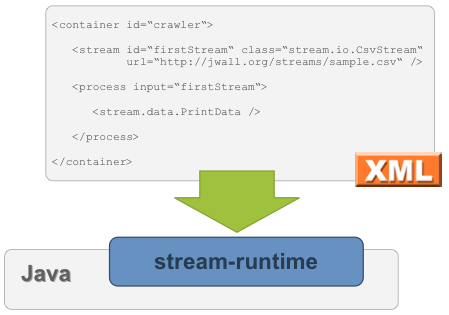
\includegraphics[scale=0.3]{graphics/quickstart-xml}
  \caption{\label{fig:quickstart}Conceptual way of executing a data flow graph that is defined in XML.}
\end{figure}

The simple example presented below, defines a single process that
reads from a CSV stream and prints out the data items to standard
output:

\begin{figure}[h!]
  \centering
  \begin{lstlisting}[language=XML]
    <container>
        <stream id="firstStream" class="stream.io.CsvStream"
                url="http://www.jwall.org/streams/sample-stream.csv" />

        <process input="firstStream">
            <PrintData />
        </process>
     </container>
  \end{lstlisting}
\end{figure}

The {\em stream-runner} required to execute this stream is a simple executable
Java archive available for download:
\begin{displaymath}
  \mbox{\url{http://download.jwall.org/streams/stream-runner.jar}}
\end{displaymath}


\subsubsection{Running a \streams Process}
The simple process defined above can be run by

\hspace{4ex}\sample{\# java -jar stream-runner.jar first-process.xml}

The process will simply read the stream in CSV-format and execute the
processor {\ttfamily PrintData} for each item obtained from the
stream.

\subsubsection{Including additional Libraries}
There exists a set pre-packaged libraries such as {\em streams-analysis}
or {\em streams-video}, which are provided at
\begin{displaymath}
  \mbox{\url{http://download.jwall.org/streams/libs/}}
\end{displaymath}
These add additional processors and stream implementations to the
\streams runtime for different domain specific intentions. To start
the \streams runtime with additional libraries, these need to be
provided on the classpath.

The following example uses the {\ttfamily MJpegImageStream} to process
a stream of video data from some URL. This stream implementation is
provided in the {\em streams-video} package.
\begin{figure}[h!]
  \centering
  \begin{lstlisting}[language=XML]
    <container>
        <stream id="video"
             class="stream.io.MJpegImageStream"
               url="http://download.jwall.org/streams/coffee.mjpeg.gz" />

        <process input="video" >

            <stream.image.DisplayImage key="data" />
            <stream.image.AverageRGB />

            <WithKeys keys="frame:*">
                 <stream.plotter.Plotter
       		         history="1000"
	                keepOpen="true"
	                keys="frame:red:avg,frame:green:avg,frame:blue:avg" />
            </WithKeys>
        </process>
    </container>
  \end{lstlisting}
  \caption{\label{fig:videoExample}Displaying an MJPEG video stream and plotting the average RGB channels.}
\end{figure}

For the libraries to be included in the path, the following command needs
to be issued to start the \streams run-time:

\hspace{4ex}\sample{\# java -cp stream-runner.jar:streams-video-0.0.1.jar $\backslash$
          stream.run video.xml}

%\section{\label{sec:streamsRuntime}The \streams Runtime}
Along with the \streams API, that is provided for implementing custom
streams or processors, the \streams framework provides a runtime
environment for running stream containers.

\subsection{Installing the \streams Runtime on Debian/RedHat}
For Debian and RPM based systems, there exists a package repository,
that provides Debian and RPM packages that can easily be installed
using the system's package managers. A step-by-step guide for setting
up the package manager on Debian and Ubuntu systems is provided in
Section \ref{sec:installDeb}. Instructions for RedHat based systems
such as RedHat, CentOS or Scientific Linux are provided in
\ref{sec:installRPM}.


\subsubsection{\label{sec:gpgKey}Signatures for Packages}
The repositories and all packages within the repository are
cryptographically signed with a GPG key with ID {\ttfamily 0x13443F4A}
to ensure their consistency. The key is available at

\sample{http://download.jwall.org/software.gpg}

The key is associated with the following information:

\sample{User ID: jwall.org Software Repository <software@jwall.org>\newline
Fingerprint: 175C 915F 51CA 8AA2 387B  E3E8 48E6 B98D 1344 3F4A}

This key needs to be added to the package management key ring of the
system (e.g. {\em apt} on Debian or {\em yum} on RedHat systems).

\subsubsection{\label{sec:installDeb}Installing on Debian/Ubuntu}
There exists a Debian/Ubuntu repository at {\ttfamily
  jwall.org}\footnote{The site \url{http://www.jwall.org/streams/} is
  the base web-site of the \streams framework.} which provides access
to the latest release versions of the \streams library.

To access this repository from within your Debian system, you'll need
create a new file {\ttfamily /etc/apt/sources.list.d/jwall.list} with
the following content:

\sample{ deb http://download.jwall.org/debian/ jwall main } 

The repositories and all packages within the repository are
cryptographically signed with a GPG key. Please see Section
\ref{sec:gpgKey} above for details on how to verify the correctness of
this key.

This key needs to be added to the APT key ring of the Debian/Ubuntu
system by running the following commands (the {\ttfamily \#} denotes
the shell prompt):

\sample{\# sudo wget http://download.jwall.org/debian/software.gpg\newline
\# sudo apt-key add software.gpg 
}

After the key and the repository have been added to the APT package
management, all that is left is to update the package list and install
the \streams environment with the following commands:

\sample{\# sudo apt-get update\newline
\# sudo apt-get install streams
}

The first command will update the package lists, the second will install
the lastest version of the {\ttfamily streams} package. After installation,
the system should be equipped with a new {\ttfamily stream.run} command
to run XML stream processes:

\sample{\# stream.run my-process.xml}

\subsubsection{\label{sec:installRPM}Installing on RedHat/CentOS/Fedora}
There exists a YUM repository at the {\ttfamily jwall.org} site, which
provides access to the latest release versions of the \streams framework
for RedHat based systems.

To access this repository from within your CentOS/RedHat system,
you'll need to create a file {\ttfamily /etc/yum.repos.d/jwall.repo}
with the following contents:

\sample{[jwall]\newline
name=CentOS-jwall - jwall.org packages for noarch\newline
baseurl=http://download.jwall.org/yum/jwall\newline
enabled=1\newline
gpgcheck=1\newline
protect=1}

The RPM packages are signed with a GPG key, please see Section
\ref{sec:gpgKey} for information how to validate this key.

To import the GPG key into your system's key ring, run the
following command as super user:

\sample{\# rpm --import http://download.jwall.org/software.gpg}

After the key has been imported your system is ready to install
the \streams package using the system's package manager, e.g.
by running

\sample{\# yum install streams}

This will download the required packages and set up the system
to provide the {\ttfamily stream.run} command to execute XML
stream processes.
\section{The \streams Core Classes}
The \streams framework provides a wide range of implementations for
data streams and processors. These are useful for reading application
data and defining a complete data flow.

In this section we provide a comprehensive overview of the classes and
implementations already available in the \streams library. These can
directly be used to design stream processes for various application
domains.

%\subsubsection{Package {\ttfamily stream.io}}
\subsection{\label{app:dataStreams}\label{api:stream:io}Data Stream Implementations}

Reading data is usually the first step in data processing. The package
{\ttfamily stream.io} provides a set of data stream implementations
for data files/resources in various formats.

All of the streams provided by this package do read from URLs, which
allows reading from files as well as from network URLs such as HTTP
urls or plain input streams (e.g. standard input).

The streams provide an iterative access to the data and use the default
\texttt{DataFactory} for creating data. They do usually share some
common parameters supported by most of the streams such as
\texttt{limit} or \texttt{username} and \texttt{password}.

\subsubsection*{Defining a Stream}
As discussed in Section \ref{sec:designingProcesses}, a stream is
defined within a container using the XML {\ttfamily stream} element,
providing a {\ttfamily url} and {\ttfamily class} attribute which
determines the source to read from and the class that should be used
for reading from that source. In addition, the definition requires a
third attribute {\ttfamily id}, which assigns the stream with a
(unique) identifier. This identifier is then used to reference the
stream as input to a process.

As a simple example, the following XML snippet defines a data stream
that reads data items in CSV format from some file URL:
\begin{figure}[h!]
        \centering
        \begin{lstlisting}{lang=xml}
           <stream  id="csv-data" class="stream.io.CsvStream"
                   url="file:/tmp/example.csv" />
        \end{lstlisting}
        \caption{Defining a CSV stream from a file.}
\end{figure}

\subsubsection*{Streaming Data from various URLs}
The \streams runtime supports a list of different URL schemes which
are provided by all Java virtual machines, e.g. {\ttfamily http} URLs
or {\ttfamily file} URLs. Custom URL schemes can also be registered
within the Java VM. As of this, the \streams runtime additionally
offers a {\ttfamily classpath:} and a {\ttfamily system:} URL scheme.

The {\ttfamily classpath:} URLs can be used to create data streams
that read from resources which are available on the classpath. This is
useful for providing example sources within custom JAR files or the
like. The following example shows how to create a stream that reads
data in JSON format from a resource {\ttfamily example.json} that is
searched for in the default classpath:
\begin{figure}[h!]
        \centering
        \begin{lstlisting}{lang=xml}
           <stream  id="json-stream"  class="stream.io.JSONStream"
                   url="classpath:/example.json" />
        \end{lstlisting}
        \caption{\label{fig:jsonStreamClasspath}Defining a JSON stream from a classpath resource.}
\end{figure}

To support streams that read data from standard input or standard
error, the library provides the {\ttfamily system:} URL schema. This
schema provides access to the system input and error streams and are
useful when piping data to a stream via the command line, e.g. by
running a command like:
\begin{figure}[h!]
\sample{\# cat data.csv | stream.run my-process.xml}
\end{figure}
To define a stream that reads from standard input, simply specify
{\ttfamily system:input} as the streams URL as shown in figure
\begin{figure}[h1]
        \centering
        \begin{lstlisting}{lang=xml}
           <stream  id="example"  class="stream.io.CsvStream"
                   url="system:input" />
        \end{lstlisting}
        \caption{\label{fig:csvStreamStdin}Defining a CSV stream that reads data from the system's standard input.}
\end{figure}

\newpage
\subsubsection{ArffStream}

This stream provides access to reading ARFF files and processing them in
a stream based fashion. ARFF is a standard format for data in the
machine learning community with its root in the
(WEKA){[}http://en.wikipedia.org/wiki/Weka\_(machine\_learning){]}
project.

\begin{figure}[h]
\begin{center}
{\renewcommand{\arraystretch}{1.2}
\textsf{
\begin{tabular}{|c|c|p{9cm}|c|} \hline
\textbf{Parameter} & \textbf{Type} & \textbf{Description} & \textbf{Required} \\ \hline  
password & String & The password for the stream URL (see username parameter) & false\\ \hline
prefix & String & An optional prefix string to prepend to all attribute names & false\\ \hline
limit & Long & The maximum number of items that this stream should deliver & false\\ \hline
username & String & The username required to connect to the stream URL (e.g web-user, database user) & false\\ \hline
\end{tabular}
 } 
 } 
\caption{Parameters of processor {\ttfamily ArffStream}}
\end{center}
\end{figure}


\subsubsection{CSVStream}

This data stream source reads simple comma separated values from a
file/url. Each line is split using a separator (regular expression).

Lines starting with a hash character (\texttt{\#}) are regarded to be
headers which define the names of the columns.

The default split expression is \texttt{(;\textbar{},)}, but this can
changed to whatever is required using the \texttt{separator} parameter.

\begin{figure}[h]
\begin{center}
{\renewcommand{\arraystretch}{1.2}
\textsf{
\begin{tabular}{|c|c|p{9cm}|c|} \hline
\textbf{Parameter} & \textbf{Type} & \textbf{Description} & \textbf{Required} \\ \hline  
keys & String[] &  & ? \\ \hline
separator & String &  & true\\ \hline
password & String & The password for the stream URL (see username parameter) & false\\ \hline
prefix & String & An optional prefix string to prepend to all attribute names & false\\ \hline
limit & Long & The maximum number of items that this stream should deliver & false\\ \hline
username & String & The username required to connect to the stream URL (e.g web-user, database user) & false\\ \hline
\end{tabular}
 } 
 } 
\caption{Parameters of processor {\ttfamily CsvStream}}
\end{center}
\end{figure}


\subsubsection{\label{api:stream:io:JSONStream}Class {\ttfamily stream.io.JSONStream}}

This data stream reads JSON objects from the source (file/url) and
returns the corresponding Data items. The stream implementation expects
each line of the file/url to provide a single object in JSON format.

\begin{figure}[h]
\begin{center}{\footnotesize
{\renewcommand{\arraystretch}{1.4}
\textsf{
\begin{tabular}{|c|c|p{9cm}|c|} \hline
\textbf{Parameter} & \textbf{Type} & \textbf{Description} & \textbf{Required} \\ \hline  
{\ttfamily id } & String &  & ? \\ \hline
{\ttfamily password } & String & The password for the stream URL (see username parameter) & false\\ \hline
{\ttfamily prefix } & String & An optional prefix string to prepend to all attribute names & false\\ \hline
{\ttfamily limit } & Long & The maximum number of items that this stream should deliver & false\\ \hline
{\ttfamily username } & String & The username required to connect to the stream URL (e.g web-user, database user) & false\\ \hline
\end{tabular}
 } 
 } 
 } 
\caption{Parameters of class {\ttfamily stream.io.JSONStream}}
\end{center}
\end{figure}

\subsubsection{LineStream}

This is a very simple stream that just reads from a URL line-by-line.
The content of the line is stored in the attribute determined by the
\texttt{key} parameter. By default the key \texttt{LINE} is used.

It also supports the specification of a simple format string that can be
used to create a generic parser to populate additional fields of the
data item read from the stream.

The parser format is:

\begin{verbatim}
  %(IP) [%(DATE)] "%(URL)"
\end{verbatim}
This will create a parser that is able to read line in the format

\begin{verbatim}
  127.0.0.1 [2012/03/14 12:03:48 +0100] "http://example.com/index.html"
\end{verbatim}
The outcoming data item will have the attribute \texttt{IP} set to
\texttt{127.0.0.1} and the \texttt{DATE} attribute set to
\texttt{2012/03/14 12:03:48 +0100}. The \texttt{URL} attribute will be
set to \texttt{http://example.com/index.html}. In addition, the
\texttt{LINE} attribute will contain the complete line string.

\begin{figure}[h]
\begin{center}{\footnotesize
{\renewcommand{\arraystretch}{1.4}
\textsf{
\begin{tabular}{|c|c|p{9cm}|c|} \hline
\textbf{Parameter} & \textbf{Type} & \textbf{Description} & \textbf{Required} \\ \hline  
{\ttfamily key } & String &  & false\\ \hline
{\ttfamily format } & String & The format how to parse each line. Elements like {\ttfamily \%(KEY)} will be detected and automatically populated in the resulting items. & false\\ \hline
{\ttfamily id } & String &  & ? \\ \hline
{\ttfamily password } & String & The password for the stream URL (see username parameter) & false\\ \hline
{\ttfamily prefix } & String & An optional prefix string to prepend to all attribute names & false\\ \hline
{\ttfamily limit } & Long & The maximum number of items that this stream should deliver & false\\ \hline
{\ttfamily username } & String & The username required to connect to the stream URL (e.g web-user, database user) & false\\ \hline
\end{tabular}
 } 
 } 
 } 
\caption{Parameters of class {\ttfamily stream.io.LineStream}}
\end{center}
\end{figure}

\subsubsection{ProcessStream}

This processor executes an external process (programm/script) that
produces data and writes that data to standard output. This can be used
to use external programs that can read files and stream those files in
any of the formats provided by the stream API.

The default format for external processes is expected to be CSV.

In the following example, the Unix command \texttt{cat} is used as an
example, producing lines of some CSV file:

\begin{verbatim}
   <Stream class="stream.io.ProcessStream"
           command="/bin/cat /tmp/test.csv"
           format="stream.io.CsvStream" />
\end{verbatim}
The process is started at initialization time and the output will be
read from standard input.

\begin{figure}[h]
\begin{center}
{\renewcommand{\arraystretch}{1.2}
\textsf{
\begin{tabular}{|c|c|p{9cm}|c|} \hline
\textbf{Parameter} & \textbf{Type} & \textbf{Description} & \textbf{Required} \\ \hline  
format & String & The format of the input (standard input), defaults to CSV & true\\ \hline
command & String & The command to execute. This command will be spawned and is assumed to output data to standard output. & true\\ \hline
\end{tabular}
 } 
 } 
\caption{Parameters of processor {\ttfamily ProcessStream}}
\end{center}
\end{figure}

\StreamSection{SQLStream}

This class implements a DataStream that reads items from a SQL database
table. The class requires a \texttt{jdbc} URL string, a username and
password as well as a \texttt{select} parameter that will select the
data from the database.

The following XML snippet demonstrates the definition of a SQL stream
from a database table called \texttt{TEST\_TABLE}:
\begin{figure}[h!]
     \begin{lstlisting}[language=XML]
         <stream class="stream.io.SQLStream"
                   url="jdbc:mysql://localhost:3306/TestDB"
              username="SA" password=""
                select="SELECT * FROM TEST_TABLE" />
     \end{lstlisting}
     \caption{\label{fig:exampleSQLStream}Example SQL streams, reading from a database.}
\end{figure}
The database connection is established using the user \texttt{SA} and no
password (empty string). The above example connects to a MySQL database.

As the SQL database drivers are not part of the streams library, you
will need to provide the database driver library for your database on
the class path.

\begin{table}[h]
\begin{center}{\footnotesize
{\renewcommand{\arraystretch}{1.4}
\textsf{
\begin{tabular}{|c|c|p{9cm}|c|} \hline
\textbf{Parameter} & \textbf{Type} & \textbf{Description} & \textbf{Required} \\ \hline  
{\ttfamily id } & String & The ID of the stream with which it is assicated to proceses.  & true \\ \hline
{\ttfamily url } & String & The JDBC database url to connect to. & true\\ \hline
{\ttfamily select } & String & The select statement to select items from the database. & true\\ \hline
{\ttfamily password } & String & The password for the stream URL (see username parameter) & false\\ \hline
{\ttfamily prefix } & String & An optional prefix string to prepend to all attribute names. & false\\ \hline
{\ttfamily limit } & Long & The maximum number of items that this stream should deliver. & false\\ \hline
{\ttfamily username } & String & The username required to connect to the stream URL (e.g web-user, database user) & false\\ \hline
\end{tabular}
 } 
 } 
 } 
\caption{Parameters of class {\ttfamily stream.io.SQLStream}.}
\end{center}
\end{table}

\subsubsection{SvmLightStream}

This stream implementation provides a data stream for the SVMlight
format. The SVMlight format is a simple \texttt{key:value} format for
compact storage of high dimensional sparse labeled data. It is a line
oriented format where each line is laid out as shown in Figure
\ref{fig:sampleSvmLight}. The keys are usually indexes, but this
stream implementation also supports string keys.
\begin{figure}[h!]
\sample{
-1.0 4:3.3 10:0.342 44:9.834 \# some comment
}
\caption{\label{fig:sampleSvmLight}A sample line of a SVMLight file.}
\end{figure}
The \texttt{\#} character starts a comment that can be provided to
each line.

\begin{table}[h]
\begin{center}{\footnotesize
{\renewcommand{\arraystretch}{1.4}
\textsf{
\begin{tabular}{|c|c|p{9cm}|c|} \hline
\textbf{Parameter} & \textbf{Type} & \textbf{Description} & \textbf{Required} \\ \hline  
{\ttfamily sparseKey } & String &  & ? \\ \hline
{\ttfamily id } & String & The ID of this string for associating it with processes. & true\\ \hline
{\ttfamily password } & String & The password for the stream URL (see username parameter) & false\\ \hline
{\ttfamily prefix } & String & An optional prefix string to prepend to all attribute names. & false\\ \hline
{\ttfamily limit } & Long & The maximum number of items that this stream should deliver. & false\\ \hline
{\ttfamily username } & String & The username required to connect to the stream URL (e.g web-user, database user) & false\\ \hline
\end{tabular}
 } 
 } 
 } 
\caption{Parameters of class {\ttfamily stream.io.SvmLightStream}.}
\end{center}
\end{table}

\paragraph{TimeStream}

This is a very simple stream that emits a single data item upon every
read. The data item contains a single attribute \texttt{@timestamp} that
contains the current timestamp (time in milliseconds).

The name of the attribute can be changed with the \texttt{key}
parameter, e.g.~to obtain the timestamp in attribute \texttt{@clock}:

\begin{verbatim}
  <Stream class="stream.io.TimeStream" key="@clock" />
\end{verbatim}


\begin{figure}[h]
\begin{center}
{\renewcommand{\arraystretch}{1.2}
\textsf{
\begin{tabular}{|c|c|p{9cm}|c|} \hline
\textbf{Parameter} & \textbf{Type} & \textbf{Description} & \textbf{Required} \\ \hline  
interval & String &  & ? \\ \hline
id & String &  & ? \\ \hline
password & String & The password for the stream URL (see username parameter) & false\\ \hline
prefix & String & An optional prefix string to prepend to all attribute names & false\\ \hline
limit & Long & The maximum number of items that this stream should deliver & false\\ \hline
username & String & The username required to connect to the stream URL (e.g web-user, database user) & false\\ \hline
\end{tabular}
 } 
 } 
\caption{Parameters of processor {\ttfamily TimeStream}}
\end{center}
\end{figure}


\newpage
\subsection{\label{api:stream:queues}Queue Implementations}
The notion of queues is similar to the definition of streams within
the \streams framework. Queues provide can be attached as sources to
processes while also allowing to be fed with data items from other
places. This allows for simple inter-process communication by
forwarding data items from one process to the queue that is read by
another different process.



\paragraph{BlockingQueue}

The \emph{BlockingQueue} provides a simple DataStream that items can be
enqueued into and read from. This allows inter-process communication
between multiple active processes to be designed using data items as
messages.

\emph{TODO:} Write details about the queuing behavior!

\begin{figure}[h]
\begin{center}
{\renewcommand{\arraystretch}{1.2}
\textsf{
\begin{tabular}{|c|c|p{9cm}|c|} \hline
\textbf{Parameter} & \textbf{Type} & \textbf{Description} & \textbf{Required} \\ \hline  
size & int &  & ? \\ \hline
id & String &  & ? \\ \hline
password & String & The password for the stream URL (see username parameter) & false\\ \hline
prefix & String & An optional prefix string to prepend to all attribute names & false\\ \hline
limit & Long & The maximum number of items that this stream should deliver & false\\ \hline
username & String & The username required to connect to the stream URL (e.g web-user, database user) & false\\ \hline
\end{tabular}
 } 
 } 
\caption{Parameters of processor {\ttfamily BlockingQueue}}
\end{center}
\end{figure}

%\paragraph{CsvUpload}

This processor simply uploads all processed items to a remote (HTTP)
URL. The upload consists of a single POST request for each item. The
POST request contains a header line and the data line as produced by the
\emph{CsvWriter}.


%\paragraph{CsvWriter}

This processor appends all processed data items to a file in CSV format.
The processor either adds all keys of the items or only a set of
previous defined keys.

As first line, the writer emits a header line with a comma separated
list of column names. This line is prepended with a \texttt{\#}
character.

The processor supports the creation of files with varying numbers of
keys/attributes. If an item is processed with a different (larger)
number of keys and the set of keys has not been defined in the
\texttt{keys} parameter, a new header will be inserted into the file,
signaling the header for the next items to be written.

By default the writer uses \texttt{,} as separator, which can be changed
by the \texttt{separator} parameter.

The following example shows a \emph{CsvWriter} writing to
\texttt{/tmp/test.csv} using the \texttt{;} as separator. Only keys
\texttt{@id} and \texttt{name} will be written:

\begin{verbatim}
  <CsvWriter url="file:/tmp/test.csv" keys="@id,name"
             separator=";" />
\end{verbatim}


\begin{figure}[h]
\begin{center}
{\renewcommand{\arraystretch}{1.2}
\textsf{
\begin{tabular}{|c|c|p{9cm}|c|} \hline
\textbf{Parameter} & \textbf{Type} & \textbf{Description} & \textbf{Required} \\ \hline  
keys & String[] & The attributes to write out, leave blank to write out all attributes. & false\\ \hline
url & String & The url to write to. & true\\ \hline
separator & String & The separator to separate columns, usually ',' & false\\ \hline
attributeFilter & String &  & ? \\ \hline
condition & String & The condition parameter allows to specify a boolean expression that is matched against each item. The processor only processes items matching that expression. & false\\ \hline
\end{tabular}
 } 
 } 
\caption{Parameters of processor {\ttfamily CsvWriter}}
\end{center}
\end{figure}

%\subsubsection{JSONWriter}

This processor writes the processed items to a file/url. The output is
written in JSON format, where a single line of JSON output is produced
for each processed item.

The result can be parsed/read using the
(JSONStream){[}JSONStream.html{]}.

\begin{figure}[h]
\begin{center}
{\renewcommand{\arraystretch}{1.2}
\textsf{
\begin{tabular}{|c|c|p{9cm}|c|} \hline
\textbf{Parameter} & \textbf{Type} & \textbf{Description} & \textbf{Required} \\ \hline  
keys & String[] & The attributes to write out, leave blank to write out all attributes. & false\\ \hline
url & String & The url to write to. & true\\ \hline
separator & String & The separator to separate columns, usually ',' & false\\ \hline
attributeFilter & String &  & ? \\ \hline
condition & String & The condition parameter allows to specify a boolean expression that is matched against each item. The processor only processes items matching that expression. & false\\ \hline
\end{tabular}
 } 
 } 
\caption{Parameters of processor {\ttfamily JSONWriter}}
\end{center}
\end{figure}

%\subsubsection{LineWriter}

This processor simply writes out items to a file in text format. The
format of the file is by default a single line for each item. Any
occurrences of new lines in the values of each item are escaped by
backslash escaping.

The following example will create a single line for each item starting
with some constant string, followed by the value of the items
\texttt{@id} attribute, a constant string \texttt{-\textgreater{}} and
the items \texttt{name} attribute:

\begin{verbatim}
  <LineWriter format="UserId: %{data.@id} -> %{data.name}"
              file="/tmp/example.out.txt"/>
\end{verbatim}


\begin{figure}[h]
\begin{center}
{\renewcommand{\arraystretch}{1.2}
\textsf{
\begin{tabular}{|c|c|p{9cm}|c|} \hline
\textbf{Parameter} & \textbf{Type} & \textbf{Description} & \textbf{Required} \\ \hline  
format & String & The format string, containing macros that are expanded for each item & true\\ \hline
file & File & Name of the file to write to. & true\\ \hline
append & boolean & Denotes whether to append to existing files or create a new file at container startup. & false\\ \hline
escapeNewlines & boolean & Whether to escape newlines contained in the attributes or not. & false\\ \hline
\end{tabular}
 } 
 } 
\caption{Parameters of processor {\ttfamily LineWriter}}
\end{center}
\end{figure}

%\subsubsection{ListDataStream}

This class implements the DataStream interface and can be used to create
a stream instance based on a collection of already available data items.

The purpose of this class is to programmatically provide a data stream
implementation, e.g.~for testing.


%\subsubsection{SQLWriter}

This processor inserts processed items into a SQL database table. At
initialization time, it checks for existence of the table and creates
the table based on the keys of the first item if the table does not
exist.

If the table exists beforehand, the table schema will be extracted and
only keys with corresponding table columns will be inserted.

The following example shows the configuration of the SQLWriter to insert
the keys \texttt{@id} and \texttt{attr1}, \texttt{attr2} into the table
\texttt{DATA}:

\begin{verbatim}
<SQLWriter keys="@id,attr1,attr2"
           url="jdbc:hsqldb:file:/tmp/test.db"
           username="SA" password=""
           table="DATA" />
\end{verbatim}
The parameters \texttt{url}, \texttt{username} and \texttt{password}
define the connection to the database, whereas the \texttt{table}
parameter defines the table into which data is to be inserted.

\subparagraph{Dropping existing Tables}

The \emph{SQLWriter} also allows to drop existing tables at
initialization time by specifying the parameter \texttt{dropTable} as
\texttt{true}.

\begin{figure}[h]
\begin{center}
{\renewcommand{\arraystretch}{1.2}
\textsf{
\begin{tabular}{|c|c|p{9cm}|c|} \hline
\textbf{Parameter} & \textbf{Type} & \textbf{Description} & \textbf{Required} \\ \hline  
table & String & The database table to insert items into. & true\\ \hline
keys & String[] & A list of attributes to insert (columns), empty string for all attributes. & false\\ \hline
dropTable & boolean &  & false\\ \hline
password & String & The password used to connect to the database. & false\\ \hline
username & String & The username used to connect to the database. & false\\ \hline
url & String & The JDBC database url to connect to. & true\\ \hline
\end{tabular}
 } 
 } 
\caption{Parameters of processor {\ttfamily SQLWriter}}
\end{center}
\end{figure}

%\subsubsection{SvmLightStream}

This stream implementation provides a data stream for the SVMlight
format. The SVMlight format is a simple \texttt{key:value} format for
compact storage of high dimensional sparse labeled data. It is a line
oriented format where each line is laid out as shown in Figure
\ref{fig:sampleSvmLight}. The keys are usually indexes, but this
stream implementation also supports string keys.
\begin{figure}[h!]
\sample{
-1.0 4:3.3 10:0.342 44:9.834 \# some comment
}
\caption{\label{fig:sampleSvmLight}A sample line of a SVMLight file.}
\end{figure}
The \texttt{\#} character starts a comment that can be provided to
each line.

\begin{table}[h]
\begin{center}{\footnotesize
{\renewcommand{\arraystretch}{1.4}
\textsf{
\begin{tabular}{|c|c|p{9cm}|c|} \hline
\textbf{Parameter} & \textbf{Type} & \textbf{Description} & \textbf{Required} \\ \hline  
{\ttfamily sparseKey } & String &  & ? \\ \hline
{\ttfamily id } & String & The ID of this string for associating it with processes. & true\\ \hline
{\ttfamily password } & String & The password for the stream URL (see username parameter) & false\\ \hline
{\ttfamily prefix } & String & An optional prefix string to prepend to all attribute names. & false\\ \hline
{\ttfamily limit } & Long & The maximum number of items that this stream should deliver. & false\\ \hline
{\ttfamily username } & String & The username required to connect to the stream URL (e.g web-user, database user) & false\\ \hline
\end{tabular}
 } 
 } 
 } 
\caption{Parameters of class {\ttfamily stream.io.SvmLightStream}.}
\end{center}
\end{table}

%\paragraph{SvmLightWriter}

The SvmLightWriter is a simple processor implementation that writes all
processed items to a file or URL using the SVMlight format. The format
supports sparse vectors and a single label attribute.

The format is described in (SvmLightStream){[}SvmLightStream.html{]}.

\begin{figure}[h]
\begin{center}
{\renewcommand{\arraystretch}{1.2}
\textsf{
\begin{tabular}{|c|c|p{9cm}|c|} \hline
\textbf{Parameter} & \textbf{Type} & \textbf{Description} & \textbf{Required} \\ \hline  
includeAnnotations & boolean &  & ? \\ \hline
keys & String[] & The attributes to write out, leave blank to write out all attributes. & false\\ \hline
url & String & The url to write to. & true\\ \hline
separator & String & The separator to separate columns, usually ',' & false\\ \hline
attributeFilter & String &  & ? \\ \hline
condition & String & The condition parameter allows to specify a boolean expression that is matched against each item. The processor only processes items matching that expression. & false\\ \hline
\end{tabular}
 } 
 } 
\caption{Parameters of processor {\ttfamily SvmLightWriter}}
\end{center}
\end{figure}

%\paragraph{TimeStream}

This is a very simple stream that emits a single data item upon every
read. The data item contains a single attribute \texttt{@timestamp} that
contains the current timestamp (time in milliseconds).

The name of the attribute can be changed with the \texttt{key}
parameter, e.g.~to obtain the timestamp in attribute \texttt{@clock}:

\begin{verbatim}
  <Stream class="stream.io.TimeStream" key="@clock" />
\end{verbatim}


\begin{figure}[h]
\begin{center}
{\renewcommand{\arraystretch}{1.2}
\textsf{
\begin{tabular}{|c|c|p{9cm}|c|} \hline
\textbf{Parameter} & \textbf{Type} & \textbf{Description} & \textbf{Required} \\ \hline  
interval & String &  & ? \\ \hline
id & String &  & ? \\ \hline
password & String & The password for the stream URL (see username parameter) & false\\ \hline
prefix & String & An optional prefix string to prepend to all attribute names & false\\ \hline
limit & Long & The maximum number of items that this stream should deliver & false\\ \hline
username & String & The username required to connect to the stream URL (e.g web-user, database user) & false\\ \hline
\end{tabular}
 } 
 } 
\caption{Parameters of processor {\ttfamily TimeStream}}
\end{center}
\end{figure}

%\paragraph{TreeStream}

This stream is a line oriented stream that expects each line to provide
a tree structure in the format

\begin{verbatim}
  ( ROOT ( A1 ( A1.1 ) ( A1.2 ) ) ( A2 ) )
\end{verbatim}


\begin{figure}[h]
\begin{center}
{\renewcommand{\arraystretch}{1.2}
\textsf{
\begin{tabular}{|c|c|p{9cm}|c|} \hline
\textbf{Parameter} & \textbf{Type} & \textbf{Description} & \textbf{Required} \\ \hline  
id & String &  & ? \\ \hline
treeAttribute & String &  & ? \\ \hline
\end{tabular}
 } 
 } 
\caption{Parameters of processor {\ttfamily TreeStream}}
\end{center}
\end{figure}



\subsection{The {\em stream-core} Processor Classes}

\subsection{Package stream.flow}

The \texttt{stream.flow} package contains processors that allow for data
flow control within a process setup. Processors in this package are
usually processor-lists, i.e.~they may provide nested processors that
are executed based on conditions.

A typical example for control flow is given with the following
\texttt{If} processor, which executes the \texttt{PrintData} processor
only, if the value of attribute \texttt{x1} is larger than 0.5.

\begin{verbatim}
   <If condition="%{data.x1} @gt 0.5">
       <PrintData />
   </If>
\end{verbatim}
Other flow control processors provide control of data queues such as
enqueuing events into other processes' queues.


\subsubsection{CreateAndEnqueue}

This processor will create a data item from the given keys and enqueue
the data item into a specified queue. This \emph{may} also result in
loops.

Macros can be used as keys.

The processor is a conditioned processor, i.e.~it supports the use of
condition expressions.

\begin{figure}[h]
\begin{center}
{\renewcommand{\arraystretch}{1.2}
\textsf{
\begin{tabular}{|c|c|p{9cm}|c|} \hline
\textbf{Parameter} & \textbf{Type} & \textbf{Description} & \textbf{Required} \\ \hline  
keys & String[] &  & ? \\ \hline
stringOnly & Boolean &  & ? \\ \hline
\end{tabular}
 } 
 } 
\caption{Parameters of processor {\ttfamily CreateAndEnqueue}}
\end{center}
\end{figure}

\subsubsection{CreateAndMultiEnqueue}

This processor will create a data item from the given keys and enqueue
the data item into the specified queues. This \emph{may} also result in
loops.

Macros can be used as keys.

The processor is a conditioned processor, i.e.~it supports the use of
condition expressions.

\begin{table}[h]
\begin{center}{\footnotesize
{\renewcommand{\arraystretch}{1.4}
\textsf{
\begin{tabular}{|c|c|p{9cm}|c|} \hline
\textbf{Parameter} & \textbf{Type} & \textbf{Description} & \textbf{Required} \\ \hline  
{\ttfamily keys } & String[] &  & ? \\ \hline
\end{tabular}
 } 
 } 
 } 
\caption{Parameters of class {\ttfamily stream.flow.CreateAndMultiEnqueue}.}
\end{center}
\end{table}

\Processor{stream.flow.Delay}

This simple processor puts a delay into the data processing. The delay
can be specified in various units with the simple time format being
specified like ``{\ttfamily 40ms}'' for specifying a delay of 40
milliseconds. Other units for \texttt{day}, \texttt{hour},
\texttt{minute} and so on work as well.

The units can also be combined as in \texttt{1 second 30ms}.

\TODO{Fix table of parameters.}
%\begin{table}[h]
%\centering
%{\footnotesize
%{\renewcommand{\arraystretch}{1.4}
%\textsf{
%\begin{tabular}{|c|c|p{9cm}|c|} \hline
%\textbf{Parameter} & \textbf{Type} & \textbf{Description} & \textbf{Required} \\ \hline  
%{\ttfamily time } & String &  & true\\ \hline
%{\ttfamily condition } & String & The condition parameter allows to specify a boolean expression that is matched against each item. The processor only processes items matching that expression. & false\\ \hline
%\end{tabular}
% } 
% }
%}
%\caption{Parameters of class {\ttfamily stream.flow.Delay}.}
%\end{table}

\Processor{Enqueue}

This processor will enqueue data items into specified queues. To
ensure mutual access to the data, the items are copied and copies are
sent to the queues. This may lead to a multiplication of data.

The processor is a conditioned processor, i.e.~it supports the use of
condition expressions. As an example, the XML snippet in Figure
\ref{fig:ex:Enqueue} will enqueue all events with a {\ttfamily color}
value equal to {\ttfamily blue} into the queue {\ttfamily blue-items}.

\begin{figure}[h!]
        \centering
        \begin{lstlisting}{lang=xml}
           <process ...>
               <Enqueue queues="blue-items" condition="%{data.color} == blue" />
           </process>
        \end{lstlisting}
        \caption{\label{fig:ex:Enqueue}The {\ttfamily Enqueue} processor combined with a condition.}
\end{figure}


\begin{table}[h]
\begin{center}{\footnotesize
{\renewcommand{\arraystretch}{1.4}
\textsf{
\begin{tabular}{|c|c|p{9cm}|c|} \hline
\textbf{Parameter} & \textbf{Type} & \textbf{Description} & \textbf{Required} \\ \hline  
{\ttfamily queues} & ServiceRef[] & A list of names that reference the target queues. & true\\ \hline
{\ttfamily condition} & Condition & A condition that is required to evaluate to {\em true} for this processor to be executed. If no condition is specified, then the processor is executed for every data item. & false\\ \hline
\end{tabular}
 } 
 } 
 } 
\caption{Parameters of class {\ttfamily stream.data.Enqueue}.}
\end{center}
\end{table}
\clearpage
\subsubsection{Every}

This processor requires a parameter \texttt{n} and will then execute all
inner processors every \texttt{n} data items, i.e.~if the number of
observed items modulo \texttt{n} equals 0.

In all other cases, the inner processors will simply be skipped.

\begin{figure}[h]
\begin{center}
{\renewcommand{\arraystretch}{1.2}
\textsf{
\begin{tabular}{|c|c|p{9cm}|c|} \hline
\textbf{Parameter} & \textbf{Type} & \textbf{Description} & \textbf{Required} \\ \hline  
n & Long &  & ? \\ \hline
\end{tabular}
 } 
 } 
\caption{Parameters of processor {\ttfamily Every}}
\end{center}
\end{figure}

\subsubsection{If}

This processor provides conditioned execution of nested processors. By
specifying a condition, all nested processors are only executed if that
condition is fulfilled.

As an example, the following will only print data items if the attribute
\texttt{x} is larger than \texttt{3.1415}:

\begin{verbatim}
  <If condition="%{data.x} @gt 3.1415">
     <PrintData />
  </If>
\end{verbatim}


\begin{figure}[h]
\begin{center}
{\renewcommand{\arraystretch}{1.2}
\textsf{
\begin{tabular}{|c|c|p{9cm}|c|} \hline
\textbf{Parameter} & \textbf{Type} & \textbf{Description} & \textbf{Required} \\ \hline  
condition & String &  & false\\ \hline
\end{tabular}
 } 
 } 
\caption{Parameters of processor {\ttfamily If}}
\end{center}
\end{figure}

\subsubsection{MultiEnqueue}

This processor will enqueue data items into the specified queues. This
\emph{may} also result in loops.

The processor is a conditioned processor, i.e.~it supports the use of
condition expressions.

\begin{figure}[h]
\begin{center}
{\renewcommand{\arraystretch}{1.2}
\textsf{
\begin{tabular}{|c|c|p{9cm}|c|} \hline
\textbf{Parameter} & \textbf{Type} & \textbf{Description} & \textbf{Required} \\ \hline  
queues & String[] &  & ? \\ \hline
\end{tabular}
 } 
 } 
\caption{Parameters of processor {\ttfamily MultiEnqueue}}
\end{center}
\end{figure}

\Processor{OnChange}

The \emph{OnChange} processor is a processor list that executes all
nested processors if some state has changed. This is similar to the
\emph{If} processor, but provides support for a process state check.

In the following example, the \emph{Message} processor is only executed
if the context variable \texttt{status} changes from \texttt{green} to
\texttt{yellow}:

\begin{verbatim}
  ...
  <OnChange from=`green` to=`yellow`>
     <Message message="Status change detected!" />
  </OnChange>
\end{verbatim}


\begin{table}[h]
\begin{center}{\footnotesize
{\renewcommand{\arraystretch}{1.4}
\textsf{
\begin{tabular}{|c|c|p{9cm}|c|} \hline
\textbf{Parameter} & \textbf{Type} & \textbf{Description} & \textbf{Required} \\ \hline  
{\ttfamily key } & String &  & true\\ \hline
{\ttfamily from } & String &  & false\\ \hline
{\ttfamily to } & String &  & false\\ \hline
{\ttfamily condition } & String &  & false\\ \hline
\end{tabular}
 } 
 } 
 } 
\caption{Parameters of class {\ttfamily stream.flow.OnChange}.}
\end{center}
\end{table}

\Processor{Skip}

This processor will simply skip all events matching a given condition.
If no condition is specified, the processor will skip all events.

The condition must be a bool expression created from numerical operators
like \texttt{@eq}, \texttt{@gt}, \texttt{@ge}, \texttt{@lt} or
\texttt{@le}. In addition to those numerical tests the \texttt{@rx}
operator followed by a regular expression can be used.

The general syntax is

\begin{verbatim}
   variable  operator  argument
\end{verbatim}
For example, the following expression will check the value of attribute
\texttt{x1} against the 0.5 threshold:

\begin{verbatim}
   %{data.x1} @gt 0.5
\end{verbatim}


\begin{table}[h]
\begin{center}{\footnotesize
{\renewcommand{\arraystretch}{1.4}
\textsf{
\begin{tabular}{|c|c|p{9cm}|c|} \hline
\textbf{Parameter} & \textbf{Type} & \textbf{Description} & \textbf{Required} \\ \hline  
{\ttfamily condition } & String & The condition parameter allows to specify a boolean expression that is matched against each item. The processor only processes items matching that expression. & false\\ \hline
\end{tabular}
 } 
 } 
 } 
\caption{Parameters of class {\ttfamily stream.flow.Skip}.}
\end{center}
\end{table}



\Package{stream.data}
This package provides processors that perform transformations or
mangling of the data items themselves. Examples for such processors are
\texttt{CreateID}, which adds a sequential ID attribute to each
processed item or the \texttt{RemoveKeys} processor which removes
attributes by name.

Other useful processors provide numerical binning
(\texttt{NumericalBinning}), setting of values in various scopes
(\texttt{SetValue}) and the like.


%\subsubsection{AddTimestamp}

This processor simply adds the current time as a UNIX timestamp to the
current data item. The default attribute/key to add is
\texttt{@timestamp}.

The value is the number of milliseconds since the epoch date, usually
1.1.1970. Using the \texttt{key} parameter, the name of the attribute to
add can be changed:

\begin{verbatim}
    &lt;stream.data.AddTimestamp key="@current-time" />
\end{verbatim}


\begin{figure}[h]
\begin{center}
{\renewcommand{\arraystretch}{1.2}
\textsf{
\begin{tabular}{|c|c|p{9cm}|c|} \hline
\textbf{Parameter} & \textbf{Type} & \textbf{Description} & \textbf{Required} \\ \hline  
key & String & The key of the timestamp attribute to add & false\\ \hline
\end{tabular}
 } 
 } 
\caption{Parameters of processor {\ttfamily AddTimestamp}}
\end{center}
\end{figure}

%\subsubsection{AsJSON}

This processor will serialize the current item into a JSON string and
add this string to the item under the key specified in the \texttt{key}
parameter. If no \texttt{key} parameter is provided, the JSON string
will be added with key \texttt{@json}.

This can for example be useful to store the JSON string of an item in a
file or database table in connection with the \emph{SQLWriter}
processor.

The following example shows the serialization into JSON and storage of
the item in a database using the \emph{AsJSON} and \emph{SQLWriter}
processor. In Addition, the \emph{CreateID} processor is used to add an
ID to the item before storing it into the database table
\texttt{data\_items}:

\begin{verbatim}
  <AsJSON key="@json" />
  <CreateID key="@id" />

  <SQLWriter url="jdbc:mysql://localhost:3306/test_db"
             username="TEST" password="TEST" table="data_items"
             keys="@id,@json" />
\end{verbatim}


\begin{figure}[h]
\begin{center}
{\renewcommand{\arraystretch}{1.2}
\textsf{
\begin{tabular}{|c|c|p{9cm}|c|} \hline
\textbf{Parameter} & \textbf{Type} & \textbf{Description} & \textbf{Required} \\ \hline  
key & String & The attribute into which the JSON string of this item should be stored. Default is '@json'. & false\\ \hline
\end{tabular}
 } 
 } 
\caption{Parameters of processor {\ttfamily AsJSON}}
\end{center}
\end{figure}

%\subsubsection{BinaryLabels}

This processor transforms items into binary labeled items with labels
with values \emph{-1.0} or \emph{+1.0}. The processor provides several
parameters that can be used for adjusting the strategy on how to map
labels.

By default the label attribute is expected to be in key \texttt{@label}.
This can be changed to the correct key name using the \texttt{label}
parameter.

\subparagraph{Mapping String labels}

In the case of labels of string type, the processor needs to be provided
with the string value of the positive class using the \texttt{positive}
parameter. Items with the label key set to the specified value for
\texttt{positive} will be flagged with a label \emph{+1.0}, all other
will be marked as \emph{-1.0}.

The following example sets up a \emph{BinaryLabels} processor mapping
all items with a label \texttt{@label} and value \texttt{SPAM} to
\emph{+1.0}. Items with any other label value are marked as \emph{-1.0}:

\begin{verbatim}
  &lt;BinaryLabels label="@label" positive="SPAM" /&gt;
\end{verbatim}
If no value for \texttt{positive} is specified, the first value for that
label key is regarded as the positive class value.

\subparagraph{Mapping Numberic Labels}

If the labels are of numberic type, the mapping can be done with a
simple threshold comparison. For this, the processor provides a
\texttt{threshold} parameter.

In the following example, items with a \texttt{@label} value higher than
\emph{0.5} are mapped to class \emph{+1.0}, all others are mapped to
class \emph{-1.0}:

\begin{verbatim}
  &lt;BinaryLabels label="@label" threshold="0.5" /&gt;
\end{verbatim}
If no threshold is specified, the default threshold of \emph{0.0} is
used.

\begin{figure}[h]
\begin{center}
{\renewcommand{\arraystretch}{1.2}
\textsf{
\begin{tabular}{|c|c|p{9cm}|c|} \hline
\textbf{Parameter} & \textbf{Type} & \textbf{Description} & \textbf{Required} \\ \hline  
threshold & Double &  & ? \\ \hline
label & String &  & ? \\ \hline
positive & String &  & ? \\ \hline
\end{tabular}
 } 
 } 
\caption{Parameters of processor {\ttfamily BinaryLabels}}
\end{center}
\end{figure}

%\subsubsection{CreateID}

This processor simply adds an incremental identifier to each processed
data item. By default, this identifier is stored as feature
\texttt{@id}, but can be used with any other name as well.

The following example creates a processor adding IDs with name
\texttt{@uid}:

\begin{verbatim}
 <CreateID key="@uid" />
\end{verbatim}
IDs are numbered starting from 0, but can also start at arbitrary
integer values:

\begin{verbatim}
 <CreateID key="@uid" start="10" />
\end{verbatim}


\begin{figure}[h]
\begin{center}
{\renewcommand{\arraystretch}{1.2}
\textsf{
\begin{tabular}{|c|c|p{9cm}|c|} \hline
\textbf{Parameter} & \textbf{Type} & \textbf{Description} & \textbf{Required} \\ \hline  
key & String &  & false\\ \hline
start & Long &  & false\\ \hline
\end{tabular}
 } 
 } 
\caption{Parameters of processor {\ttfamily CreateID}}
\end{center}
\end{figure}

%\subsubsection{Lookup}

This processor provides a way to use a
\texttt{stream.service.LookupService} and add the provided dataitem to
the processed dataitem. For example

\begin{verbatim}
  <Lookup key="testkey" lookup-ref="lookupService" />
\end{verbatim}
will use the \texttt{stream.service.LookupService} lookupService to
lookup the key testkey and merge the to dataitems.

This is useful, e.g.~when static information are needed.

It is also possible to use macros as key.

\begin{figure}[h]
\begin{center}
{\renewcommand{\arraystretch}{1.2}
\textsf{
\begin{tabular}{|c|c|p{9cm}|c|} \hline
\textbf{Parameter} & \textbf{Type} & \textbf{Description} & \textbf{Required} \\ \hline  
key & String &  & false\\ \hline
\end{tabular}
 } 
 } 
\caption{Parameters of processor {\ttfamily Lookup}}
\end{center}
\end{figure}

%\subsubsection{MapKeys}

This processor provides a way to map keys (feature names) to other
values. This is sometimes required to match special processors that rely
on specific feature names:

\begin{verbatim}
  <MapKeys from="labelAttribute" to="@label" />
\end{verbatim}
A more complex setting can be used by specifying the map in a
\texttt{key=value} file, e.g.~stored as \texttt{my-map.txt}. With such a
file, the processor can be specified as:

\begin{verbatim}
  <MapKeys map="my-map.txt" />
\end{verbatim}
where the \texttt{my-map.txt} file may look like

\begin{verbatim}
  attr1=sepalLength
  attr2=sepalWidth
  ...
\end{verbatim}
which will map the keys according to the map.

\begin{figure}[h]
\begin{center}
{\renewcommand{\arraystretch}{1.2}
\textsf{
\begin{tabular}{|c|c|p{9cm}|c|} \hline
\textbf{Parameter} & \textbf{Type} & \textbf{Description} & \textbf{Required} \\ \hline  
from & String &  & ? \\ \hline
to & String &  & ? \\ \hline
map & String &  & false\\ \hline
mapping & Map & A list of key mappings. & true\\ \hline
\end{tabular}
 } 
 } 
\caption{Parameters of processor {\ttfamily MapKeys}}
\end{center}
\end{figure}

%\subsubsection{MapValue}

This processor provides a way to map values of a specific feature to
integer IDs, starting with 1 as first ID. The processor will maintain a
map of value-to-IDs and extend that map for new values.

\begin{verbatim}
  <MapValueToID key="data" />
\end{verbatim}


\begin{figure}[h]
\begin{center}
{\renewcommand{\arraystretch}{1.2}
\textsf{
\begin{tabular}{|c|c|p{9cm}|c|} \hline
\textbf{Parameter} & \textbf{Type} & \textbf{Description} & \textbf{Required} \\ \hline  
key & String &  & false\\ \hline
\end{tabular}
 } 
 } 
\caption{Parameters of processor {\ttfamily MapValueToID}}
\end{center}
\end{figure}

%\subsubsection{MapValue}

This processor provides a way to map values of a specific feature onto
other values. For example, mapping all labels \texttt{0.0} to the value
\texttt{-1.0} can be done using

\begin{verbatim}
  <MapValues key="@label" from="0.0" to="-1.0" />
\end{verbatim}
This is useful, e.g.~when required to map labels or other categorical
data to different values.

A more complex setting can be used by specifying the map in a
\texttt{key=value} file, e.g.~stored as \texttt{my-map.txt}. With such a
file, the processor can be specified as:

\begin{verbatim}
  <MapValues key="@label" map="my-map.txt" />
\end{verbatim}
where the \texttt{my-map.txt} file may look like

\begin{verbatim}
  false=-1.0
  true=1.0
\end{verbatim}
which will map the string values \texttt{true} and \texttt{false}
according to the map.

\begin{figure}[h]
\begin{center}
{\renewcommand{\arraystretch}{1.2}
\textsf{
\begin{tabular}{|c|c|p{9cm}|c|} \hline
\textbf{Parameter} & \textbf{Type} & \textbf{Description} & \textbf{Required} \\ \hline  
from & String &  & ? \\ \hline
to & String &  & ? \\ \hline
key & String &  & ? \\ \hline
map & String &  & ? \\ \hline
\end{tabular}
 } 
 } 
\caption{Parameters of processor {\ttfamily MapValues}}
\end{center}
\end{figure}

%\subsubsection{NumericalBinning}

This processor transforms a numeric attribute into a discrete nominal
attribute by creating bins and mapping all values onto a bin. This can
be regarded as a simple interval-based discretization.

The \emph{NumericalBinning} processor requires a \texttt{minimum},
\texttt{maximum} and \texttt{bins} parameter to be set. It will then
compute equi-distant interval from these values and will replace each
value by a string denoting the interval/bin it was mapped to.

By default, the \emph{NumericalBinning} will discretize all numeric
attributes, i.e.~all keys that refer to an Integer, Long, Float or
Double value. If the \texttt{keys} parameter is provided, only the
attributes listed in \texttt{keys} are discretized.

The following example shows the numerical binning for attribute
\texttt{x1}:

\begin{verbatim}
    &lt;NumericalBinning keys="x1" minimum="0.0" maximum="10.0" bins="10" /&gt;
\end{verbatim}


\begin{figure}[h]
\begin{center}
{\renewcommand{\arraystretch}{1.2}
\textsf{
\begin{tabular}{|c|c|p{9cm}|c|} \hline
\textbf{Parameter} & \textbf{Type} & \textbf{Description} & \textbf{Required} \\ \hline  
key & String &  & ? \\ \hline
minimum & Double &  & ? \\ \hline
maximum & Double &  & ? \\ \hline
bins & Integer &  & ? \\ \hline
keys & String[] &  & ? \\ \hline
\end{tabular}
 } 
 } 
\caption{Parameters of processor {\ttfamily NumericalBinning}}
\end{center}
\end{figure}

%\subsubsection{PrintData}

This processor will simply print out the processed elements to the
standard output. As the processor is a conditioned processor, it can
also be used to print only specific items, matching a given condition.

The following example shows a processor that will only print items with
no key \texttt{x1}:

\begin{verbatim}
  <PrintData condition="%{data.x1} == null" />
\end{verbatim}


\begin{figure}[h]
\begin{center}
{\renewcommand{\arraystretch}{1.2}
\textsf{
\begin{tabular}{|c|c|p{9cm}|c|} \hline
\textbf{Parameter} & \textbf{Type} & \textbf{Description} & \textbf{Required} \\ \hline  
condition & String & The condition parameter allows to specify a boolean expression that is matched against each item. The processor only processes items matching that expression. & false\\ \hline
\end{tabular}
 } 
 } 
\caption{Parameters of processor {\ttfamily PrintData}}
\end{center}
\end{figure}

%\subsubsection{RandomBinaryLabel}

This operator simply adds a random label (either -1.0 or +1.0) to
processed data items. The labels are distributed normally.

The \texttt{key} parameter allows for specifying the label attribute
name, which by default is considered to be \texttt{@label}:

\begin{verbatim}
 <RandomBinaryLabel key="@label" />
\end{verbatim}


\begin{figure}[h]
\begin{center}
{\renewcommand{\arraystretch}{1.2}
\textsf{
\begin{tabular}{|c|c|p{9cm}|c|} \hline
\textbf{Parameter} & \textbf{Type} & \textbf{Description} & \textbf{Required} \\ \hline  
seed & Long &  & ? \\ \hline
key & String &  & ? \\ \hline
\end{tabular}
 } 
 } 
\caption{Parameters of processor {\ttfamily RandomBinaryLabel}}
\end{center}
\end{figure}

%\subsubsection{RemoveAttributes}

This processors provides the possibility to remove a set of features
from each processed data item. The list can be specified by setting the
\texttt{keys} parameter to the list of features to be removed:

\begin{verbatim}
  <RemoveAttributes keys="attr1,attr2,attr3" />
\end{verbatim}
The key strings will be splitted at each comma and will be trimmed,
i.e.~the list above will have the same effect as the following:

\begin{verbatim}
  <RemoveAttributes keys="attr1, attr2 , attr3" />
\end{verbatim}


\begin{figure}[h]
\begin{center}
{\renewcommand{\arraystretch}{1.2}
\textsf{
\begin{tabular}{|c|c|p{9cm}|c|} \hline
\textbf{Parameter} & \textbf{Type} & \textbf{Description} & \textbf{Required} \\ \hline  
keys & String[] &  & ? \\ \hline
\end{tabular}
 } 
 } 
\caption{Parameters of processor {\ttfamily RemoveKeys}}
\end{center}
\end{figure}

%\subsubsection{RemoveZeroes}

This processor will remove any values which equal 0 in the numerical
sense. This can be used to remove a large number of features to create a
sparse item:

\begin{verbatim}
  <RemoveZeroes />
\end{verbatim}
Special attributes, such as \texttt{@label} or similar are left
untouched.


%\subsubsection{RenameKey}

This processor simply renames a single attribute. The attribute value
will be removed from the data item and added with the new key,
overwriting any existing entry with that new key.

Example:

\begin{verbatim}
   <RenameKey key="myKey" to="myNewName" />
\end{verbatim}


\begin{figure}[h]
\begin{center}
{\renewcommand{\arraystretch}{1.2}
\textsf{
\begin{tabular}{|c|c|p{9cm}|c|} \hline
\textbf{Parameter} & \textbf{Type} & \textbf{Description} & \textbf{Required} \\ \hline  
from & String & The old name of the key. & true\\ \hline
to & String & The new name of the key. & true\\ \hline
condition & String & The condition parameter allows to specify a boolean expression that is matched against each item. The processor only processes items matching that expression. & false\\ \hline
\end{tabular}
 } 
 } 
\caption{Parameters of processor {\ttfamily RenameKey}}
\end{center}
\end{figure}

%\subsubsection{SelectKeys}

This processor can be used to select a subset of keys from the current
data item. The result of this will be a data item that has all keys
removed except for those that have been selected by the \texttt{keys}
parameter.

The \texttt{keys} parameter also allows for specifying keys with
wildcards \texttt{*} and \texttt{?}. In the following example all
attributes that start with \texttt{user:} will be selected, but not
\texttt{user:gender}:

\begin{verbatim}
 <SelectKeys keys="user:*,!user:gender" />
\end{verbatim}


\begin{figure}[h]
\begin{center}
{\renewcommand{\arraystretch}{1.2}
\textsf{
\begin{tabular}{|c|c|p{9cm}|c|} \hline
\textbf{Parameter} & \textbf{Type} & \textbf{Description} & \textbf{Required} \\ \hline  
keys & String[] &  & ? \\ \hline
remove & Boolean &  & ? \\ \hline
\end{tabular}
 } 
 } 
\caption{Parameters of processor {\ttfamily SelectKeys}}
\end{center}
\end{figure}

%\Processor{SetValue}

This processors allows for setting a feature to a single, constant
value:
\begin{figure}[h!]
\centering
\begin{lstlisting}{lang=xml}
  <SetValue key="attribute1" value="abc" />
\end{lstlisting}
\end{figure}

\begin{table}[h]
\begin{center}{\footnotesize
{\renewcommand{\arraystretch}{1.4}
\textsf{
\begin{tabular}{|c|c|p{9cm}|c|} \hline
\textbf{Parameter} & \textbf{Type} & \textbf{Description} & \textbf{Required} \\ \hline  
{\ttfamily value } & String &  & ? \\ \hline
{\ttfamily key } & String & The name of the attribute to set. & true \\ \hline
{\ttfamily scope } & String[] & The scope determines where the variable will be set. Valid scopes are {\ttfamily process}, {\ttfamily data}. The default scope is {\ttfamily data}. & false\\ \hline
{\ttfamily condition } & String & The condition parameter allows to specify a boolean expression that is matched against each item. The processor only processes items matching that expression. & false\\ \hline
\end{tabular}
 } 
 } 
 } 
\caption{Parameters of class {\ttfamily stream.data.SetValue}.}
\end{center}
\end{table}

%\subsubsection{TrimKeys}

This operator removes leading and trailing whitespaces from all keys of
a data item, i.e.~the item

\begin{verbatim}
 x1  =1.0
\end{verbatim}
will be transformed to

\begin{verbatim}
 x1=1.0
\end{verbatim}
as the key ``\texttt{x1}'' will be renamed to ``\texttt{x1}'' (without
the quotes).


\Processor{WithKeys}

This processor is a processor list that executes one or more inner
processors. It creates a copy of the current data item with all
attributes matching the list of specified keys. Then all nested
processors are applied to that copy and the copy is merged back into
the original data item.

If any of the nested data items returns \emph{null}, this processor will
also return \emph{null}.

The \texttt{keys} parameter of this processor allows for specifying a
comma separated list of keys and key-patterns using simple wildcards
\texttt{*} and \texttt{?} as shown in Figure \ref{fig:withKeys}. If
the {\ttfamily keys} parameter is not provided, then the inner
processors will be provided with a complete copy of the current data
item.

\begin{figure}[h!]
\begin{lstlisting}{lang=xml}
      <process ...>
          <WithKeys keys="x1,user:*,!user:id">
             <PrintData />
          </WithKeys>
      </process>
\end{lstlisting}
\caption{\label{fig:withKeys}Selects only attribute {\ttfamily x1},
  all attributes starting with {\ttfamily user:} but not attribute
  {\ttfamily user:id} and executes the {\ttfamily PrintData} processor
  for this selection of attributes.}
\end{figure}


\begin{table}[h]
\begin{center}{\footnotesize
{\renewcommand{\arraystretch}{1.4}
\textsf{
\begin{tabular}{|c|c|p{9cm}|c|} \hline
\textbf{Parameter} & \textbf{Type} & \textbf{Description} & \textbf{Required} \\ \hline  
{\ttfamily keys } & String[] & A list of filter keys selecting the attributes that should be provided to the inner processors. & false\\ \hline
{\ttfamily merge } & Boolean & Indicates whether the outcome of the inner processors should be merged into the input data item, defaults to true. & false\\ \hline
\end{tabular}
 } 
 } 
 } 
\caption{Parameters of class {\ttfamily stream.data.WithKeys}.}
\end{center}
\end{table}


\subsection{Package stream.parser}

When processing streams of data each single data item may contain
additional information that needs to be extracted into more detailed
attributes or into other value types.

The \texttt{stream.parser} package provides a set of parsing processors,
that usually act upon on or more keys and extract information from the
attributes denoted by those keys.

For example the \texttt{ParseDouble} processor will parse double values
from all strings that are denoted in its \texttt{keys} parameter. Other
parsers in this package are for example the \texttt{ParseJSON},
\texttt{Timestamp} or the \texttt{NGrams} processor.


\Processor{NGrams}

This parser processor will create n-grams from a specified attribute of
the processed item and will add all the n-grams and their frequency to
the item. By default the processor creates n-grams of length 3.

To not overwrite any existing keys, the n-gram frequencies can be
prefixed with a user-defined string using the \texttt{prefix} parameter.

The following example shows an \emph{NGram} processor that will create
5-grams of the string found in key \texttt{text} and add their frequency
to the items with a prefix of \texttt{5gram}:

\begin{verbatim}
  <NGrams n="5" key="text" prefix="5gram" />
\end{verbatim}


\begin{table}[h]
\begin{center}{\footnotesize
{\renewcommand{\arraystretch}{1.4}
\textsf{
\begin{tabular}{|c|c|p{9cm}|c|} \hline
\textbf{Parameter} & \textbf{Type} & \textbf{Description} & \textbf{Required} \\ \hline  
{\ttfamily key } & String & The attribute which is to be split into n-grams & true\\ \hline
{\ttfamily n } & Integer & The length of the n-grams that are to be created & true\\ \hline
{\ttfamily prefix } & String & An optional prefix that is to be prepended for all n-gram names before these are added to the data item & false\\ \hline
\end{tabular}
 } 
 } 
 } 
\caption{Parameters of class {\ttfamily stream.parser.NGrams}.}
\end{center}
\end{table}

\subsubsection{ParseDouble}

This simple processor parses all specified keys into double values. If a
key cannot be parsed to a double it will be replaced by
\emph{Double.NaN}.

The processor will be applied for all keys of an item unless the
\texttt{keys} parameter is used to specify the keys/attributes that
should be transformed into double values.

The following example shows a \emph{ParseDouble} processor that converts
the attributes \texttt{x1} and \texttt{x2} into double values:

\begin{verbatim}
  <ParseDouble keys="x1,x2" />
\end{verbatim}
\subparagraph{Different Default Value}

The \texttt{default} parameter allows for specifying a different value
than the default \emph{Double.NaN} value. The following example converts
all values to their double representation and defaults to 0.0 if parsing
as double fails:

\begin{verbatim}
  <ParseDouble default="0.0" />
\end{verbatim}


\begin{figure}[h]
\begin{center}
{\renewcommand{\arraystretch}{1.2}
\textsf{
\begin{tabular}{|c|c|p{9cm}|c|} \hline
\textbf{Parameter} & \textbf{Type} & \textbf{Description} & \textbf{Required} \\ \hline  
default & Double & The default value to set if parsing fails & false\\ \hline
keys & String[] & The keys/attributes to perform parsing on & true\\ \hline
\end{tabular}
 } 
 } 
\caption{Parameters of processor {\ttfamily ParseDouble}}
\end{center}
\end{figure}

\Processor{Timestamp}

This processor parses the date time from an attribute using a specified
format string and stores the parsed time as a long value into the
\texttt{@timestamp} key by default.

The processor requires at least a \texttt{format} and a \texttt{from}
parameter. The \texttt{format} specifies a date format to parse the time
from. The \texttt{from} parameter determines the key attribute from
which the date is to be parsed.

The following example shows a timestamp parser that parses the
\texttt{DATE} key using the format \texttt{yyyy-MM-dd-hh:mm:ss}. The
resulting timestamp (milliseconds UNIX time) is stored under key
\texttt{@time}:

\begin{verbatim}
  <Timestamp key="@time" format="yyyy-MM-dd-hh:mm:ss"
             from="DATE" />
\end{verbatim}


\begin{table}[h]
\begin{center}{\footnotesize
{\renewcommand{\arraystretch}{1.4}
\textsf{
\begin{tabular}{|c|c|p{9cm}|c|} \hline
\textbf{Parameter} & \textbf{Type} & \textbf{Description} & \textbf{Required} \\ \hline  
{\ttfamily key } & String &  & false\\ \hline
{\ttfamily format } & String & The date format string used for parsing. & true\\ \hline
{\ttfamily from } & String & The key/attribute from which the timestamp should be parsed. & true\\ \hline
{\ttfamily timezone } & String & The timezone that the processed data is assumed to refer to. & false\\ \hline
\end{tabular}
 } 
 } 
 } 
\caption{Parameters of class {\ttfamily stream.parser.ParseTimestamp}.}
\end{center}
\end{table}


\end{appendix}